\chapter{\acf{MCM}}
\section{Note sulla probabilit\`a}
\subsection{Errore probabile}
Per una variabile casuale $X$ distribuita normalmente con
\begin{itemize}
\item media $\mu$;
\item varianza $\sigma$;
\end{itemize}
si ha che per
\begin{equation*}
  r = 0.6745\sigma
\end{equation*}
vale
\begin{eqnarray*}
  \prob{\mu-r<X<\mu+r} &=& 0.5\\
  \prob{\abs{X-\mu}<r} &=& 0.5\\
  \prob{\abs{X-\mu}>r} &=& 0.5.
\end{eqnarray*}
Quindi valori di $X$ che deviano da $\mu$ pi\`u o meno di $r$ hanno
stesse probabilit\`a ed $r$ identifica l'errore pi\`u probabile di
una distribuzione normale.

\subsection{Teorema del limite centrale delle probabilit\`a}
Si considerino $N$ variabili casuali $X_1,X_2,\dots,X_N$ indipendenti e distribuite
identicamente. Quindi con stessa media e stessa varianza:
\begin{eqnarray*}
  \expected{X_1}=\expected{X_2}=\dots=\expected{X_N}&=&m\\
  \variance{X_1}=\variance{X_2}=\dots=\variance{X_N}&=&b^2.
\end{eqnarray*}

Si consideri la somma di queste variabili casuali:
\begin{equation*}
  Y = X_1+X_2+\cdots+X_N
\end{equation*}
si ha che
\begin{eqnarray*}
  \expected{Y}&=&\expected{X_1+X_2+\cdots+X_N}=Nm\\
  \variance{Y}&=&\variance{X_1+X_2+\cdots+X_N}=Nb^2.
\end{eqnarray*}

Si consideri adesso una variabile casuale $Z$ distribuita normalmente
con parametri:
\begin{eqnarray*}
  \mu&=&Nm\\
  \sigma&=&b\sqrt{N}
\end{eqnarray*}
con funzione di densit\`a denotata da $p_Z(x)$.

Il teorema centrale del limite afferma che per $N$ grande, e per ogni
intervallo $(x_1,x_2)$ vale:
\begin{equation}\label{eq:tcl}
  \prob{x_1<Y<x_2}\approx\int_{x_1}^{x_2}p_Z(x) \md x
\end{equation}
quindi la somma di un numero elevato di variabili
casuali aventi distribuzione identica \`e distribuita normalmente con
media e varianza uguali a quelle originali (anche se queste non erano
distribuite normalmente).

\section{\acf{MCM}}
Supponendo di dover calcolare una certa quantit\`a sconosciuta $m$,
dobbiamo trovare una variabile casuale $X$ tale che:
\begin{equation*}
  \expected{X} = m.
\end{equation*}
Avendo tale distribuzione, con varianza uguale a:
\begin{equation*}
  \variance{X} = b^2
\end{equation*}
 \`e possibile mostrare i seguenti passaggi.

Si considerino $N$ variabili casuali $X_1,X_2,\dots,X_N$ con
distribuzione identica a quella di $X$. Quindi per il teorema del
limite centrale~\eqref{eq:tcl} si ha, per $N$ sufficientemente grande, che la
distribuzione della somma
\begin{equation*}
  Y=X_1+X_2+\cdots+X_N
\end{equation*}
\`e distribuita normalmente con parametri
\begin{eqnarray*}
  \mu &=& Nm\\
  \sigma&=&b\sqrt{N}.
\end{eqnarray*}

Per la regola dei \emph{tre sigma} si ha:
\begin{eqnarray*}
  \prob{\mu-3\sigma < Y <\mu +3\sigma}&\approx& 0.997\\
  \prob{Nm-3b\sqrt{N} < Y < Nm+3b\sqrt{N}}&\approx& 0.997
\end{eqnarray*}
dividendo per $N$:
\begin{eqnarray*}
  \prob{m-\frac{3b}{\sqrt{N}} < \frac{Y}{N} <
    m+\frac{3b}{\sqrt{N}}}&\approx& 0.997\\
  \prob{\abs{\frac{Y}{N}-m} <\frac{3b}{\sqrt{N}}}&\approx& 0.997
\end{eqnarray*}
e quindi:
\begin{equation}\label{eq:mc}
  \prob{\abs{\frac{1}{N}\sum_{i=1}^NX_i-m} <\frac{3b}{\sqrt{N}}}\approx 0.997.
\end{equation}

L'equazione~\eqref{eq:mc} afferma che, se viene estratto un campione per ogni
variabile casuale $X_i$, la media aritmetica di questi valori \`e
approssimativamente uguale a $m$. Inoltre, l'errore di questa
approssimazione \`e pari a $3b/\sqrt{N}$, che tende a $0$ al crescere
di $N$. \`E possibile ridurre ulteriormente l'incertezza
aumentando il numero $k$ di sigma usati per l'approssimazione e
quindi valutando l'errore $kb/\sqrt{N}$.

In realt\`a, poich\'e le variabili casuali $X_i$ hanno la stessa
distribuzione di $X$, \`e sufficiente estrarre $N$ campioni da $X$ per
giungere alle stesse conclusioni.
Il \ac{MCM} \`e costituito
dal seguente procedimento da adattare secondo i casi:
\begin{enumerate}
\item si trova la distribuzione $X$ con media la quantit\`a desiderata
  $m$ e varianza $b^2$;
\item si estraggono $N$ campioni di $X$, in numero grande abbastanza
  da avere un errore piccolo a piacere;
\item la media aritmetica di tali $N$ campioni d\`a il valore
  approssimato di $m$.
\end{enumerate}
Quindi il problema diventa quello di ricavare la distribuzione $X$ o,
comunque, gli $N$ campioni distribuiti in accordo con $X$.

Se vogliamo caratterizzare pi\`u nel dettaglio l'errore commesso
prendendo $N$ campioni, possiamo ricorrere all'\emph{errore
  probabile}. Ponendo $k=0.6745$ si ha che 
\begin{equation*}
  \prob{\abs{\frac{1}{N}\sum_{i=1}^NX_i-m} <\frac{0.6745\cdot b}{\sqrt{N}}}\approx 0.5
\end{equation*}
e quindi 
\begin{equation*}
  r_N = \frac{0.6745\cdot b}{\sqrt{N}}
\end{equation*}
 indica di quanto si discosta mediamente il
valore della media dei campioni $\frac{1}{N}\sum_{i=1}^NX_i$ dalla misura cercata
$m$. Tale valore caratterizza l'errore assoluto
\begin{equation*}
\abs{\frac{1}{N}\sum_{i=1}^NX_i-m}  
\end{equation*}
commesso prendendo $N$ campioni.

\subsection{\acf{MCI}}
Il \ac{MCM} \`e utile per simulare fenomeni che hanno un alto grado di
incertezza negli input o un alto numero di gradi di libert\`a.

Una
applicazione specifica \`e \ac{MCI}. Integrare numericamente una
funzione che ha
molte dimensioni o che ha caratteristiche particolari, come quella di
figura~\ref{fig:func}, pu\`o diventare un problema estremamente
difficile. Monte Carlo pu\`o essere utile in questi casi per ottenere
un'approssimazione dell'integrale.
\begin{figure}[h!]
  \centering
  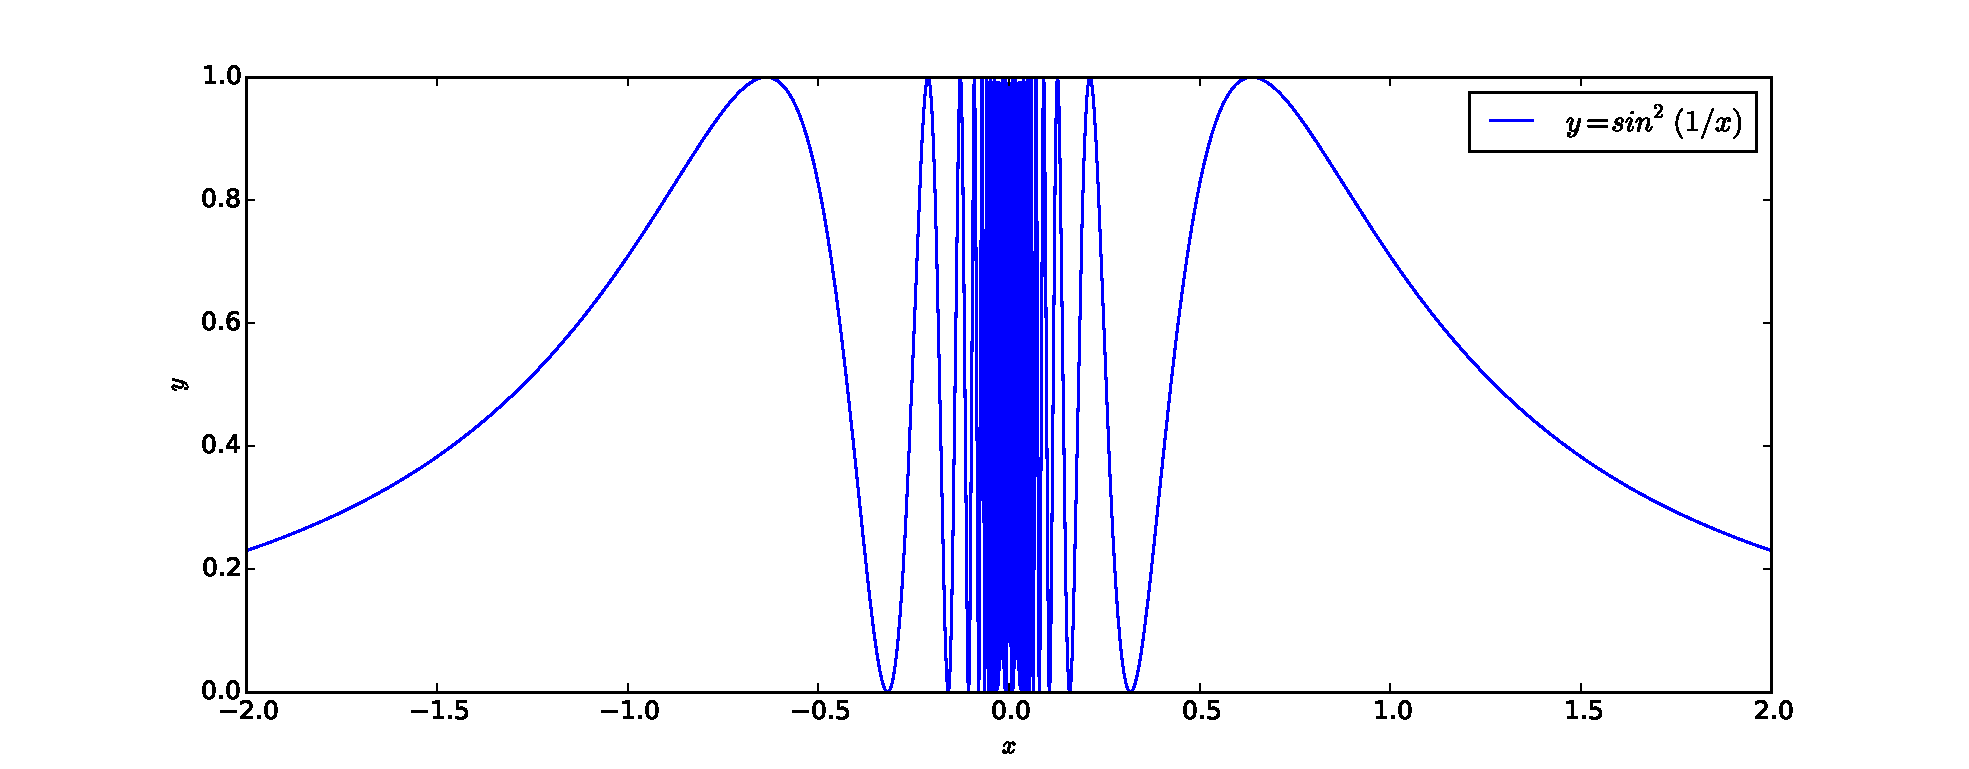
\includegraphics[width=\textwidth]{montecarlo1.pdf}
  \caption{Funzione $y=sen^2(1/x)$ non ben definita intorno allo $0$.}
  \label{fig:func}
\end{figure}

Consideriamo la funzione:
\begin{equation*}
  f(x)\equiv sen^2(\frac{1}{x}),
\end{equation*}
\`e sempre compresa tra $0$ e $1$, non \`e definita per
$x=0$ e inoltre intorno allo $0$ si addensano le oscillazioni. La
funzione integrale
\begin{equation*}
  I(x) \equiv \int_0^x f(x') \md x'
\end{equation*}
\`e l'area sotto la curva $f(x)$ compresa tra $0$ e $x$. Ha sempre valore finito
compreso tra $0<I(x)<X$, ma non \`e semplice da calcolare vicino
all'origine.

Se scegliamo due numeri casuali
\begin{itemize}
\item  $u$ uniformemente distribuito tra $0$ e $x$;
\item $v$ uniformemente distribuito tra $0$ e $1$;
\end{itemize}
si ha che la probabilit\`a che il punto $h = (u, v)$, nella
figura~\ref{fig:func}, sia sotto la curva 
$f(x)$ \`e $I(x)/x$, ossia il rapporto tra l'area sotto la curva e
l'area limitata da $0$ e $x$ nelle
ascisse e da $0$ e $1$ nelle ordinate.

Il punto $h$ \`e sotto la
curva se $v<f(u)$. Quindi, prendendo un campione sufficientemente
grande di $N$ punti e contando gli $M$ punti che stanno sotto la
curva\footnote{Usando la disequazione $v<f(u)$.}, \`e possibile
stimare il valore di $I(x)$ con:
\begin{equation*}
  I(x)\approx \frac{M}{N}x.
\end{equation*}

In figura~\ref{fig:int} \`e possibile vedere l'approssimazione di
$I(x)$ usando \ac{MCI} con $10000$ campioni. In appendice \`e
riportato il codice\footnote{Notare che le figure
  sono state create impostando \codei{numCampioni} e \codei{numPuntiX}
  uguali a 10000, mentre nel codice sono uguali a 1000 per velocizzare
  il processo in caso di esecuzione di questo.} \emph{Python} usato
per creare i plot delle
figure~\ref{fig:func} e~\ref{fig:int}.
\begin{figure}[h!]
  \centering
  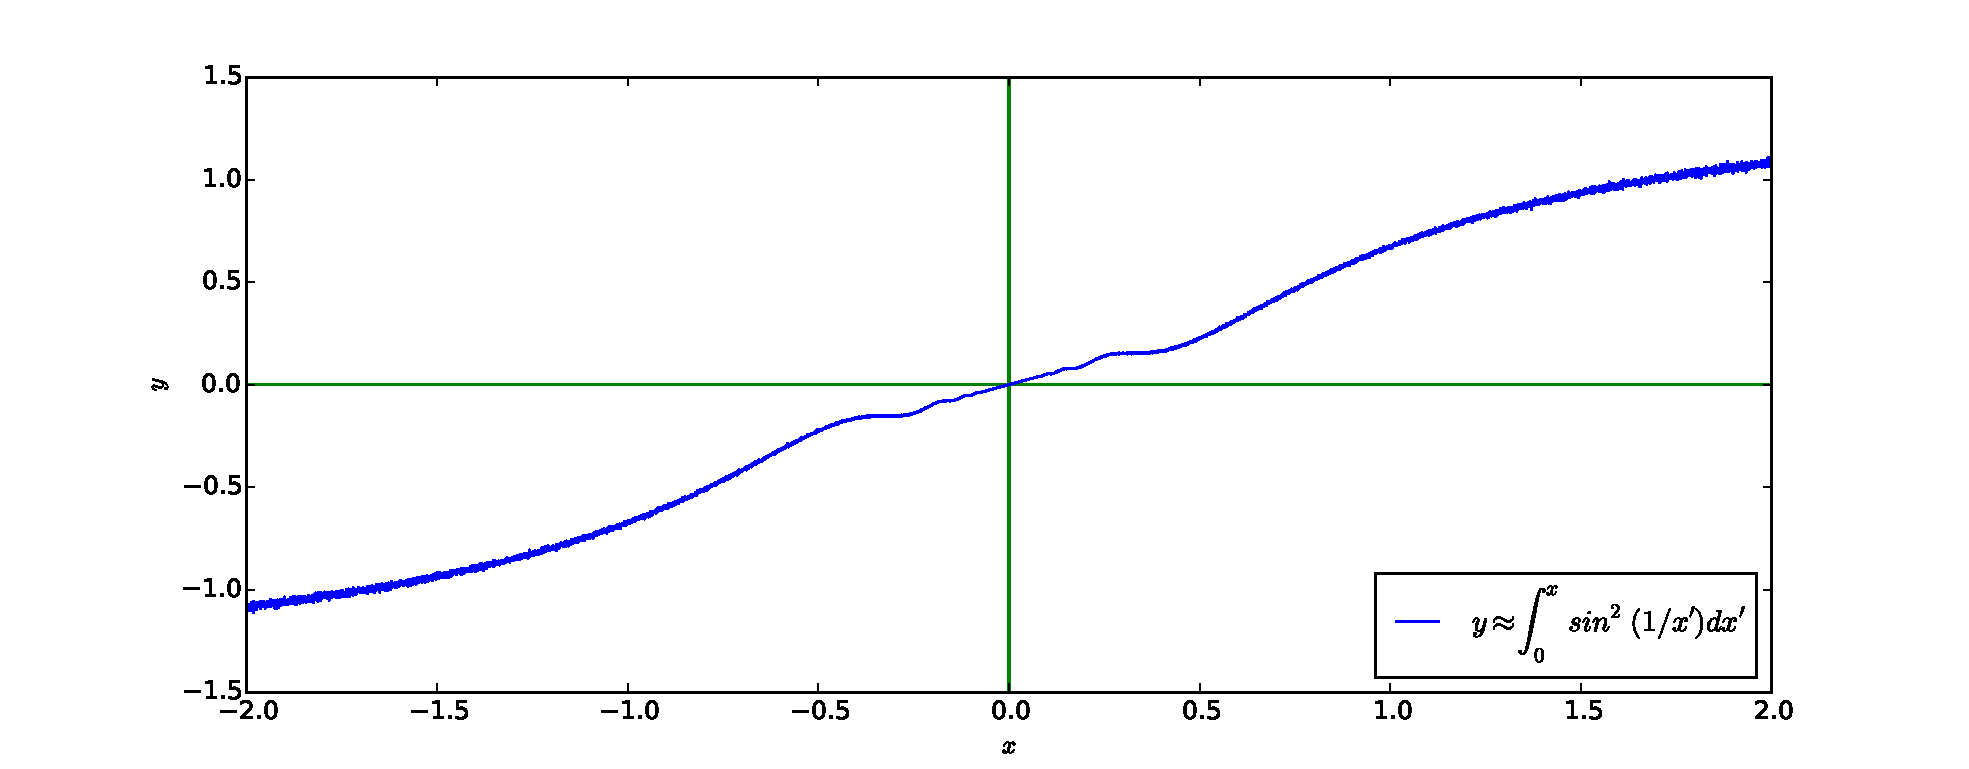
\includegraphics[width=\textwidth]{montecarlo2.pdf}
  \caption{Approssimazione della funzione integrale $y=\int_0^x sen^2(1/x')\md x'$, ottenuta
    con \ac{MCI} con $N=10000$ campioni.}
  \label{fig:int}
\end{figure}

\newpage
\section{Appendice}
\lstinputlisting[style=customPy]{montecarlo.py}

